% Drawing 122/01-5 -- folder 122, batch 01, archive page 16 (PDF page 17).
% Transcription: au milieu de la page, premier diagramme en perspective : les lettres $S$, $W$, $T$ en haut, $P$, $Q$, $M$, $R$, $N$, $t$ au milieu, $T$ et $S$ repassés, $(s,t)$, $\emptyset$ et $t$ en bas, reliées par des flèches montantes dont plusieurs épaisses ; des ovales au crayon entourent des groupes de lettres ; deux plages hachurées, à gauche et à droite en bas.
% Kind: arrow diagram in perspective (lattice of inclusions), with hatched regions. Method 2 (schematic redraw from the facsimile). Status: partial.
% Notes: The letters are placed as on the page and the arrows drawn between the places where they start and end on the page: M to the upper left, P to S (top), a faint line from s to S, P to W and M to P (hooked), R to P (heavy), Q to the upper left (heavy), Q to T, t to T, R to Q, N to Q, N to t, T (heavy letter) to M, T to R, S (heavy letter) to R, S to N, (s,t) to T and to S, the empty set to (s,t), S down to the lower t (heavy), and a dashed stroke from that t up to a small T on the right. Under R, a small vertical equality sign and T x S. Four pencil ovals surround P and R, M and T, R and Q, S and N; two scribbled hatchings at the lower left (with two small s) and lower right. Partial: the hooks, dots and small crosses on several arrows (M to P, P to W, T to R, S to N carry a hook or a cross) are not drawn; arrow heads retraced on the page are drawn once; the ovals and hatchings are placed by eye; which letter each arrow reaches is read from its direction, and several are doubtful (Q's upper-left arrow ends in the blank between W and T; M's ends near the small s). Overlaid 2026-11-12 (Opus 5.5) on a 400 dpi colour render: letters and arrows match the page within about a unit; the oval round R and Q was too short and too flat in its tilt and is corrected (35 degrees); the hatching at the lower right was drawn sloping the wrong way and about 5 units low, and is now strokes rising to the right over the place of the scribble; both hatchings remain schematic (the page has zigzag scribbles). Redrawn 2026-11-12 (issue 128): to check again. 2026-11-13, Claude Opus 5.5, overlay check (issue 147): not compiled (no TeX in the session); the TikZ rasterised and laid over the 236 ppi colour scan (rendered at 350 dpi), with an ink/pencil separation of the crop to follow the faint strokes. Redrawn element by element on the scan: every arrow between the points where its ink starts and ends (several were 1 to 2 units off), with what it carries on the page: the hooked tails (P to W, M to P, R to Q, T to R, (s,t) to S, S to N: a small c; N to Q, S to R, T to M, (s,t) to T, the empty set to (s,t): a U or J; Q's upper-left arrow and R to P: a short upturn), the heavy dots (on P to W, M to P, Q's upper-left arrow, R to Q, T to R, S to R), the small ring on R to P, the cross on T to M and the asterisk on S to N; the arrow from S down to the lower t ends in a right-angle head; the dashed stroke starts from a small c and ends at the foot of the small T. The four pencil ovals are now the open curves they are on the page, through points read on them: round P and R (open where P to W crosses it), round R and Q (its lower edge broken), round S and N (open above N), and the one round M and T in three pieces (open at the M to P hook and below T), with two short pencil strokes between it and the first oval. Letters moved onto their ink (W, M, T x S and the vertical equality sign were 1 unit off). Every element lies on the ink to within about 1 unit. Still differs, hence partial: the two hatchings are scribbles; the one at the lower left is drawn as a zigzag through the turning points of its loops (its strokes are curved and doubled on the page), the one at the lower right as its separate straight strokes with the long curve under them; the head of the arrow from (s,t) to S is a blot on the page, drawn as a small head.
% Coordinates: 1 unit = 1 mm = 1/100 of the crop width (bbox in page fractions: [0.32, 0.235, 0.7, 0.405]).
% Redrawn by Claude (claude-fable-5-2), issue #128, 2026-11-12; not checked by a human; not compiled (no TeX in the session).
% Overlaid by Claude (claude-opus-5-5) 2026-11-12 (issue #128): rasterised from its own coordinates over the colour facsimile and checked or corrected. Not compiled. Status: partial.
% Revised by Claude Opus 5.5 (claude-opus-5-5), issue #147, 2026-11-13: overlay check on the colour scan; not checked by a human; not compiled (no TeX in the session).
% Rights: reproduces part of the work -- behind RENDER_TRANSCRIPTS, never published by itself.
\documentclass[tikz,border=3pt]{standalone}
\usepackage{amsmath,amssymb}
\usetikzlibrary{patterns,arrows.meta}
\tikzset{pencil/.style={black!45}, struck/.style={black!35}, mpt/.style={circle,draw,inner sep=1.3pt}, pt/.style={circle,fill,inner sep=0.9pt}, opt/.style={circle,draw,fill=white,inner sep=1.1pt}}
\begin{document}
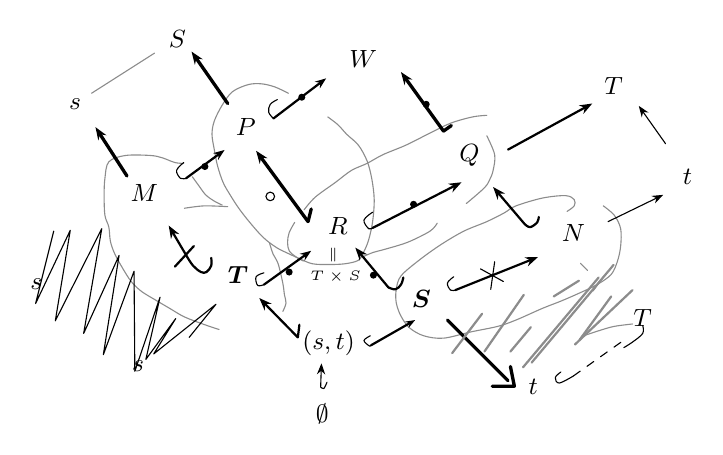
\begin{tikzpicture}[x=1mm,y=1mm,line cap=round,line join=round,font=\scriptsize]
% letters
\node[inner sep=1pt] at (23.6,-2.2) {\small $S$};
\node[inner sep=1pt] at (10.6,-10.5) {\small $s$};
\node[inner sep=1pt] at (47.2,-4.7) {\small $W$};
\node[inner sep=1pt] at (32.3,-13.4) {\small $P$};
\node[inner sep=1pt] at (19.4,-21.8) {\small $M$};
\node[inner sep=1pt] at (60.7,-17) {\small $Q$};
\node[inner sep=1pt] at (79,-8.2) {\small $T$};
\node[inner sep=1pt] at (88.4,-19.7) {\small $t$};
\node[inner sep=1pt] at (44,-26) {\small $R$};
\node[inner sep=1pt] at (73.9,-26.9) {\small $N$};
\node[inner sep=1pt] at (31.3,-32.2) {\small $\boldsymbol{T}$};
\node[inner sep=1pt] at (54.6,-35.2) {\small $\boldsymbol{S}$};
\node[inner sep=1pt] at (42.8,-40.8) {\small $(s,t)$};
\node[inner sep=1pt] at (42,-49.8) {\small $\emptyset$};
\node[inner sep=1pt] at (68.8,-46.4) {\small $t$};
\node[inner sep=1pt] at (82.7,-37.6) {\small $T$};
\node[inner sep=1pt] at (5.7,-33.3) {\small $s$};
\node[inner sep=1pt] at (18.6,-43.7) {\small $s$};
\node[inner sep=1pt] at (43.4,-29.7) {\tiny $\parallel$};
\node[inner sep=1pt] at (43.7,-32.4) {\tiny $T \times S$};
% pencil ovals, each through points read on it (open where the page leaves them open)
\draw[pencil] plot[smooth, tension=0.55] coordinates {(37.7,-9.1) (36,-8.3) (34.3,-7.9) (32.6,-8) (30.6,-8.9) (29.3,-10.6) (28.3,-12.6) (28,-14.3) (28.3,-16.3) (28.7,-18.3) (29.4,-20.4) (30.3,-22) (31.4,-23.7) (32.8,-25.5) (34.5,-27.4) (36.2,-28.7) (37.8,-29.5) (39.1,-30.1) (40.75,-30.75) (42.8,-30.85) (44.9,-30.75) (46.6,-30.3) (47.3,-29.2) (47.9,-27.7) (48.4,-25.4) (48.6,-22.6) (48.3,-20) (47.7,-17.7) (46.6,-15.7) (45.1,-14.3) (44,-13.1) (42.7,-12.1)};
\draw[pencil] plot[smooth, tension=0.55] coordinates {(39.7,-23.9) (41.1,-22.3) (43.7,-20.4) (45.7,-18.9) (47.7,-18) (49.7,-16.9) (52.6,-15.7) (55.4,-14.3) (58.3,-12.9) (61.1,-12.1) (62.9,-11.9)};
\draw[pencil] plot[smooth, tension=0.55] coordinates {(62.9,-14.5) (63.9,-16.9) (63.7,-18.9) (63.3,-20) (62.6,-21.1) (60.3,-23.1)};
\draw[pencil] plot[smooth, tension=0.55] coordinates {(38.5,-25.5) (37.8,-26.8) (37.6,-28) (37.8,-29.1) (38.7,-29.9) (39.6,-30.4)};
\draw[pencil] plot[smooth, tension=0.55] coordinates {(47.3,-29.8) (48.5,-29.3) (50,-28.9) (52.9,-28) (55.7,-26.6) (56.6,-25.6)};
\draw[pencil] plot[smooth, tension=0.55] coordinates {(73.1,-24.1) (74,-23.4) (74,-22.6) (72.9,-22.1) (70,-22.4) (66.6,-23.4) (65.1,-24.3) (62.9,-25.4) (60,-26.6) (57.1,-28.3) (54.3,-30.3) (52,-32.3) (51.4,-34) (51.4,-35.7) (52,-37.4) (53.1,-38.9) (54.9,-39.9) (57.4,-40.2) (60.9,-39.4) (64.3,-38.7) (66.6,-37.9) (70,-36.4) (72.3,-35.5) (74.6,-34.5) (76.9,-33.4) (78.7,-32.1) (79.5,-30.4) (79.9,-28.5) (79.9,-26.3) (79.1,-24.6) (77.7,-23.4)};
\draw[pencil] plot[smooth, tension=0.55] coordinates {(24.4,-18) (23.3,-17.9) (21.7,-17.3) (20.2,-17) (17,-17) (14.9,-17.8) (14.4,-19.9) (14.3,-22.1) (14.4,-24.6) (14.9,-26.1) (15.1,-27.9) (15.7,-29.6) (17,-31.9) (17.9,-33.2) (19.1,-34.3) (20.9,-35.4) (22.6,-36.4) (24.5,-37.5) (27.1,-38.5) (28.9,-39.1)};
\draw[pencil] plot[smooth, tension=0.55] coordinates {(25.5,-19.7) (26.3,-20.8) (27.2,-22) (28.3,-22.8) (29.3,-23.3)};
\draw[pencil] plot[smooth, tension=0.55] coordinates {(24.5,-23.7) (27,-23.4) (30,-23.5)};
\draw[pencil] plot[smooth, tension=0.55] coordinates {(35.3,-28.1) (35.75,-29.5) (36.4,-30.75) (37,-33.25) (37.2,-34.7) (37.4,-35.75) (37,-36.8)};
% faint line from s towards S
\draw[pencil] (12.7,-9.1) -- (20.7,-4);
% arrows (hooks, dots, rings and crosses as on the page)
\draw[-{Stealth[length=1.6mm]},very thick] (17.2,-19.6) -- (13.2,-13.4);
\draw[-{Stealth[length=1.6mm]},very thick] (30,-10.4) -- (25.4,-3.8);
\draw plot[smooth, tension=0.6] coordinates {(36.3,-9.9) (35.4,-10.5) (35.2,-11.5) (35.8,-12.3)};
\draw[-{Stealth[length=1.4mm]},thick] (35.8,-12.3) -- (42.5,-7.2);
\node[pt] at (39.4,-9.6) {};
\draw plot[smooth, tension=0.6] coordinates {(24.4,-17.9) (23.5,-18.9) (24,-19.9) (24.7,-19.9)};
\draw[-{Stealth[length=1.4mm]},thick] (24.7,-19.9) -- (29.6,-16.3);
\node[pt] at (27.1,-18.4) {};
\draw[-{Stealth[length=1.6mm]},very thick] (40.2,-25.4) -- (33.6,-16.4);
\draw[very thick] (40.2,-25.4) -- (40.6,-23.8);
\node[opt] at (35.4,-22.2) {};
\draw[-{Stealth[length=1.6mm]},very thick] (57.4,-13.9) -- (52,-6.4);
\draw[very thick] (57.4,-13.9) -- (58.4,-13.2);
\node[pt] at (55.2,-10.5) {};
\draw[-{Stealth[length=1.6mm]},thick] (65.6,-16.25) -- (76.3,-10.4);
\draw[-{Stealth[length=1.4mm]}] (85.6,-15.5) -- (82.2,-10.7);
\draw plot[smooth, tension=0.6] coordinates {(48.4,-24.2) (47.3,-25.2) (47.9,-26.3) (48.4,-26.2)};
\draw[-{Stealth[length=1.6mm]},thick] (48.4,-26.2) -- (59.7,-20.4);
\node[pt] at (53.6,-23.2) {};
\draw[-{Stealth[length=1.6mm]},thick] (67.7,-25.7) -- (63.7,-21);
\draw[thick] plot[smooth, tension=0.6] coordinates {(67.7,-25.7) (68.4,-26.1) (69.3,-25.5) (69.5,-24.8)};
\draw[-{Stealth[length=1.4mm]}] (78.3,-25.4) -- (85.3,-22);
\draw[-{Stealth[length=1.6mm]},thick] (24.8,-29.8) -- (22.5,-25.9);
\draw[thick] plot[smooth, tension=0.6] coordinates {(24.8,-29.8) (25.6,-31) (26.6,-31.8) (27.3,-31.8) (27.9,-31) (27.9,-30)};
\draw[thick] (25.7,-28.5) -- (23.3,-31.1);
\draw plot[smooth, tension=0.6] coordinates {(34.6,-31.9) (33.6,-32.4) (33.8,-33.5) (34.6,-33.4)};
\draw[-{Stealth[length=1.4mm]},thick] (34.6,-33.4) -- (40.6,-29.1);
\node[pt] at (37.8,-31.8) {};
\draw[-{Stealth[length=1.6mm]},thick] (50.4,-33.75) -- (46.2,-28.7);
\draw[thick] plot[smooth, tension=0.6] coordinates {(50.4,-33.75) (51.3,-34) (52,-33.4) (52.3,-32.5)};
\node[pt] at (48.5,-32.2) {};
\draw plot[smooth, tension=0.6] coordinates {(58.7,-32.4) (57.9,-33.2) (58.3,-34.1) (58.9,-34.1)};
\draw[-{Stealth[length=1.6mm]},thick] (58.9,-34.1) -- (69.4,-29.9);
\draw (63.9,-30.5) -- (63.4,-34);
\draw (62.1,-31.4) -- (65,-33);
\draw[-{Stealth[length=1.6mm]},thick] (38.9,-40.1) -- (34,-35.1);
\draw[thick] (38.9,-40.1) -- (39.1,-38.5);
\draw plot[smooth, tension=0.6] coordinates {(48.1,-39.9) (47.3,-40.5) (48,-41.2) (48.2,-41.1)};
\draw[-{Stealth[length=1.2mm]},thick] (48.2,-41.1) -- (53.8,-37.9);
\draw[-{Stealth[length=1.4mm]}] (41.8,-46.4) -- (41.9,-43.4);
\draw plot[smooth, tension=0.6] coordinates {(41.8,-46.4) (42.2,-46.6) (42.6,-45.8)};
\draw[very thick] (57.9,-37.9) -- (65.6,-45.6);
\draw[very thick] (63.6,-46.3) -- (66.4,-46.3) -- (65.9,-43.8);
% dashed stroke from the lower t up to the small T
\draw plot[smooth, tension=0.6] coordinates {(72.3,-44.5) (71.6,-45.2) (72.1,-45.9) (73.9,-45)};
\draw[dashed] (73.9,-45) -- (80.1,-40.6);
\draw plot[smooth, tension=0.6] coordinates {(80.3,-41.4) (81.4,-40.7) (82.7,-39.6) (82.7,-38.6)};
% hatching at the lower left: a zigzag scribble, tops and bottoms read on the page
\draw (7.9,-26.6) -- (5.6,-35.8) -- (10,-26.5) -- (8.1,-38) -- (14,-26.3) -- (11.7,-39.6) -- (16.2,-29.7) -- (14.2,-42.3) -- (18.1,-31.7) -- (18.2,-44.4) -- (21.4,-35) -- (19.6,-42.9) -- (23.4,-37.7) -- (20.6,-42.2) -- (28.5,-35.9) -- (25.1,-40.1);
% hatching at the lower right: separate strokes rising to the right
\draw[pencil,thick] (58.5,-42.1) -- (62.3,-37.1);
\draw[pencil,thick] (62.6,-41.9) -- (67.6,-34.7);
\draw[pencil,thick] (65.9,-41.9) -- (68.5,-38.8);
\draw[pencil,thick] (71.4,-34.9) -- (74.6,-32.9);
\draw[pencil,thick] (67.5,-43.9) -- (77.1,-32.5);
\draw[pencil,thick] (68.6,-43.3) -- (79,-30.9);
\draw[pencil,thick] (74.1,-41) -- (81.4,-34.1);
\draw[pencil,thick] (74.7,-40.4) -- (78.7,-34.9);
\draw[pencil] plot[smooth, tension=0.55] coordinates {(74.9,-40) (77.3,-39.2) (79.1,-38.7) (81.4,-38.4)};
\draw[pencil] (76.4,-34.2) -- (77.8,-32.3);
\draw[pencil] (74.8,-30.7) -- (75.7,-31.6);
\end{tikzpicture}
\end{document}
